\documentclass[12pt, a4paper]{article}
\usepackage[UTF8]{ctex}
\usepackage{amsmath, amssymb}
\usepackage{graphicx}
\usepackage{geometry}
\usepackage{fancyhdr}
\usepackage{booktabs}
\usepackage{array}
\usepackage{float}
\usepackage{enumitem}
\usepackage{xcolor}
\usepackage{titlesec}
\usepackage{textcomp}
\usepackage{tikz}
\usepackage{listings}
\usepackage{caption}
\usepackage{tocloft}
\usetikzlibrary{positioning, arrows.meta}
\usepackage{graphicx}

% Figures live in ../media relative to this file
\graphicspath{{../media/}}

% ===== Hyperlink settings =====
\usepackage[hidelinks]{hyperref}
\hypersetup{
    pdfauthor={},
    pdftitle={Automatic 3D Terrain Construction System Based on ROS and MoveIt}
}

% ===== Code style settings =====
\definecolor{codebg}{RGB}{248,248,248}
\definecolor{codeframe}{RGB}{200,200,200}
\definecolor{keywordcolor}{RGB}{0,0,200}
\definecolor{stringcolor}{RGB}{200,0,0}
\definecolor{commentcolor}{RGB}{0,128,0}

\lstdefinestyle{pythonstyle}{
    language=Python,
    basicstyle=\small\ttfamily,
    keywordstyle=\color{keywordcolor}\bfseries,
    stringstyle=\color{stringcolor},
    commentstyle=\color{commentcolor},
    numbers=left,
    numberstyle=\tiny\color{gray},
    stepnumber=1,
    numbersep=5pt,
    showstringspaces=false,
    breaklines=true,
    frame=single,
    tabsize=4,
    xleftmargin=2pt,
    xrightmargin=2pt,
    backgroundcolor=\color{codebg},
    rulecolor=\color{codeframe}
}

\lstnewenvironment{pythoncode}[1][]
{
    \lstset{style=pythonstyle, title=#1}
}
{}

% ===== Page layout =====
\geometry{a4paper, margin=2.5cm}
\setlength{\parindent}{2em}
\setlength{\parskip}{0.5em}
\setlength{\headheight}{14.5pt}
\addtolength{\topmargin}{-2.5pt}

% ===== Header and footer =====
\pagestyle{fancy}
\fancyhf{}
\fancyhead[C]{\textbf{Robotics I Final Project}}
\fancyfoot[C]{\thepage}
\renewcommand{\headrulewidth}{0.4pt}

% ===== Title format =====
\titleformat{\section}{\Large\bfseries\centering}{\thesection}{1em}{}
\titleformat{\subsection}{\large\bfseries}{\thesubsection}{1em}{}
\titleformat{\subsubsection}{\normalsize\bfseries}{\thesubsubsection}{1em}{}

% ===== Table of contents format =====
\renewcommand{\contentsname}{Contents}
\renewcommand{\figurename}{Figure}
\renewcommand{\tablename}{Table}
\renewcommand{\cftsecfont}{\normalfont}
\renewcommand{\cftsecpagefont}{\normalfont}
\renewcommand{\cftsubsecfont}{\normalfont}
\renewcommand{\cftsubsecpagefont}{\normalfont}

% ===== Document info =====
\title{\vspace{2cm}\Huge\textbf{Automatic 3D Terrain Construction System Based on ROS and MoveIt}\\[0.5em]}
\author{Project Team}
\date{June 23, 2026}

\begin{document}

\maketitle
\thispagestyle{empty}
\newpage

\setcounter{page}{1}
\tableofcontents
\newpage

% ============================================================
% Chapter 1: Project Overview and Task Goals
% ============================================================
\section{Project Overview and Task Goals}

This project builds an automated robotic system based on ROS Noetic and MoveIt for automatic 3D terrain construction.

\subsection{Operating Environment}

\begin{itemize}
    \item ROS Noetic + MoveIt + RViz
\end{itemize}

\subsection{Actuator}

\begin{itemize}
    \item Franka Emika Panda 7-joint robot arm
\end{itemize}

% ===== 插入机械臂结构图 =====
\begin{figure}[H]
    \centering
    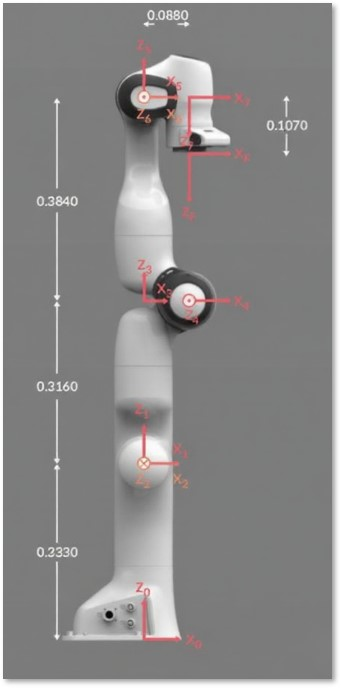
\includegraphics[width=0.45\textwidth]{structure.jpg}
    \caption{Franka Emika Panda robot arm structure}
    \label{fig:panda_structure}
\end{figure}

% ===== 插入 D-H 参数表图 =====
\begin{figure}[H]
    \centering
    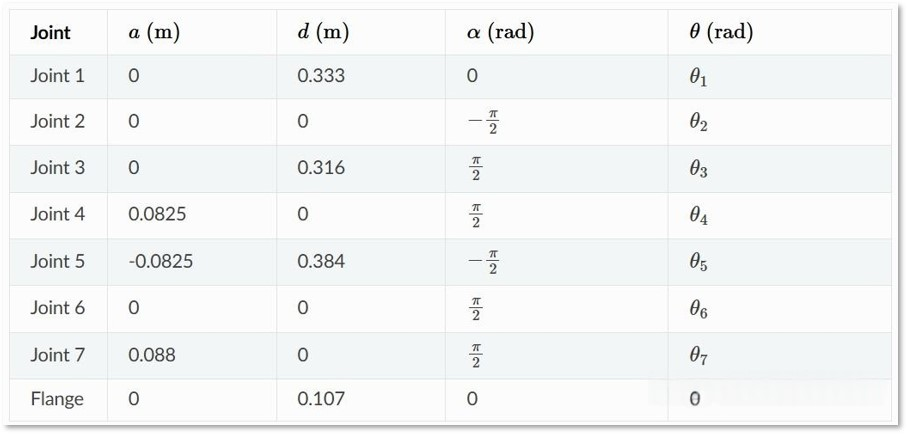
\includegraphics[width=\textwidth]{DH.jpg}
    \caption{Denavit-Hartenberg (D-H) parameters of the Panda arm}
    \label{fig:dh_parameters}
\end{figure}

The Franka Emika Panda is a 7-degree-of-freedom anthropomorphic robot arm. 
\textbf{Figure~\ref{fig:panda_structure}} shows the physical structure and joint layout, 
while \textbf{Figure~\ref{fig:dh_parameters}} presents the corresponding D-H parameter table, 
which defines the kinematic relationships between successive links. 
These parameters are essential for forward and inverse kinematics computations 
in the MoveIt planning pipeline.

\subsection{Core Tasks}

\begin{itemize}
    \item Simple contour to $32 \times 32$ matrix
    \item Maximum stacking height: 8 layers
    \item Hundreds of high-precision pick-and-place cycles
    \item Imitate real terrain
\end{itemize}

% ============================================================
% Chapter 2: System Design
% ============================================================
\section{System Design}

The system adopts a three-layer architecture: Driver Layer, Recognition Layer, and Control Layer.

\subsection{Driver Layer}

The Driver Layer is based on ROS + MoveIt + RViz and relies on the \texttt{panda\_moveit} package, responsible for robot arm motion control and visualization.

The launch file \texttt{terrain\_builder\_demo.launch} launches the entire system with the following configuration:

\begin{itemize}
    \item Robot arm type: Franka Emika Panda
    \item Mode: Simulation
    \item Controller: OMPL $\to$ RRT + collision detection
\end{itemize}

\begin{pythoncode}[terrain\_builder\_demo.launch]
<!-- Launch Panda + MoveIt core -->
<include file="$(find panda_moveit_config)/launch/demo.launch">
  <arg name="arm_id" value="panda" />
  <arg name="pipeline" value="ompl" />
  <arg name="moveit_controller_manager" value="fake" />
  <arg name="fake_execution_type" value="interpolate" />
</include>

<!-- Launch RViz with terrain-optimized config -->
<node name="rviz" pkg="rviz" type="rviz"
      args="-d terrain_builder.rviz" />

<!-- Run terrain builder after initialization -->
<node name="terrain_builder"
      pkg="panda_moveit_config"
      type="terrain_builder.py"
      output="screen"
      launch-prefix="bash -c 'sleep 3; exec $0 $@'" />
\end{pythoncode}

This launch file accomplishes three key tasks:
\begin{enumerate}
    \item Load the Panda robot arm URDF model and the Open Motion Planning Library (OMPL) kinematics solver
    \item Launch RViz with a visualization configuration optimized for terrain building
    \item Start the core control node \texttt{terrain\_builder.py} after a 3-second delay
\end{enumerate}

\subsection{Recognition Layer}

The core module of the Recognition Layer is \texttt{contour\_to\_heightmap.py}, whose main functions include:

\begin{itemize}
    \item Convert simple contour maps to matrices
    \item Generate a $32 \times 32$ terrain matrix
\end{itemize}

\subsection{Control Layer}

The core module of the Control Layer is \texttt{terrain\_builder.py}, whose main functions include:

\begin{itemize}
    \item Launch file startup
    \item Robot arm control
    \item Block control
\end{itemize}

\begin{figure}[H]
    \centering
    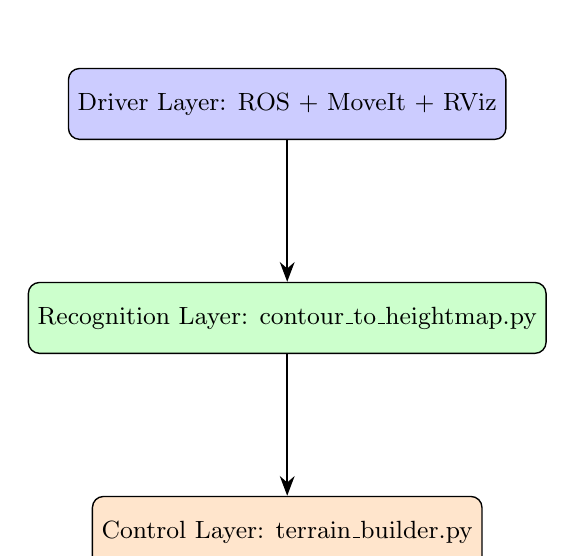
\begin{tikzpicture}[
        node distance=1.8cm,
        auto,
        font=\small,
        block/.style={rectangle, rounded corners, draw, minimum width=4.2cm, minimum height=0.9cm, align=center, line width=0.5pt},
        arrow/.style={-{Stealth[length=2.5mm]}, thick}
    ]
        \node[block, fill=blue!20] (driver) {Driver Layer: ROS + MoveIt + RViz};
        \node[block, fill=green!20, below=1.8cm of driver] (recog) {Recognition Layer: contour\_to\_heightmap.py};
        \node[block, fill=orange!20, below=1.8cm of recog] (control) {Control Layer: terrain\_builder.py};
        
        \draw[arrow] (driver) -- (recog);
        \draw[arrow] (recog) -- (control);
    \end{tikzpicture}
    \caption{System Three-Layer Architecture}
    \label{fig:architecture}
\end{figure}

% ============================================================
% Chapter 3: Recognition Layer
% ============================================================
\section{Recognition Layer}

The Recognition Layer is responsible for converting contour terrain maps into height matrices that the robot arm can recognize.

\subsection{Input and Output}

\begin{itemize}
    \item \textbf{Input}: Colored contour map (colors represent heights)
    \item \textbf{Processing}: Grid sampling + color-height matching
    \item \textbf{Output}: $32 \times 32$ matrix with max element up to 8
\end{itemize}

\subsection{Color-Height Mapping}

The system predefines 8 contour levels with corresponding colors:

\begin{pythoncode}[contour\_to\_heightmap.py: Color Mapping]
CONTOUR_COLORS_BGR = {
    1: (255, 0, 0),      # Blue
    2: (0, 255, 0),      # Green
    3: (0, 255, 255),    # Yellow
    4: (0, 165, 255),    # Orange
    5: (0, 0, 255),      # Red
    6: (255, 0, 255),    # Magenta
    7: (255, 255, 0),    # Cyan
    8: (128, 0, 128),    # Purple
}
\end{pythoncode}

\subsection{Core Processing Function}

The conversion from image to height matrix is implemented by the \texttt{image\_to\_heightmap} function:

\begin{pythoncode}[contour\_to\_heightmap.py: Image to Height Matrix]
def image_to_heightmap(image, grid_size=8, num_levels=8):
    """Convert a contour image to a 2D heightmap matrix."""
    h, w = image.shape[:2]
    heightmap = np.zeros((grid_size, grid_size), dtype=np.int32)
    cell_w = float(w) / grid_size
    cell_h = float(h) / grid_size

    for i in range(grid_size):
        for j in range(grid_size):
            # Sample the pixel at the center of each grid cell
            px = int((j + 0.5) * cell_w)
            py = int((i + 0.5) * cell_h)
            bgr = tuple(image[py, px])
            level = _color_to_level(bgr)
            if level > 0:
                heightmap[i, j] = level
    return heightmap
\end{pythoncode}

This function divides the image into an $N \times N$ grid, samples the center pixel of each cell, and determines the height level through color matching.

\subsection{Technical Workflow}

\begin{enumerate}
    \item Import contour map
    \item Pixel sampling
    \item Color-height mapping
    \item Generate \texttt{heightmap.npy}
\end{enumerate}

\begin{figure}[H]
    \centering
    \begin{minipage}{0.45\textwidth}
        \centering
        
\includegraphics[width=\textwidth]{contour_map.png}
        \caption{Input: Colored contour map}
        \label{fig:contour}
    \end{minipage}
    \hfill
    \begin{minipage}{0.45\textwidth}
        \centering
        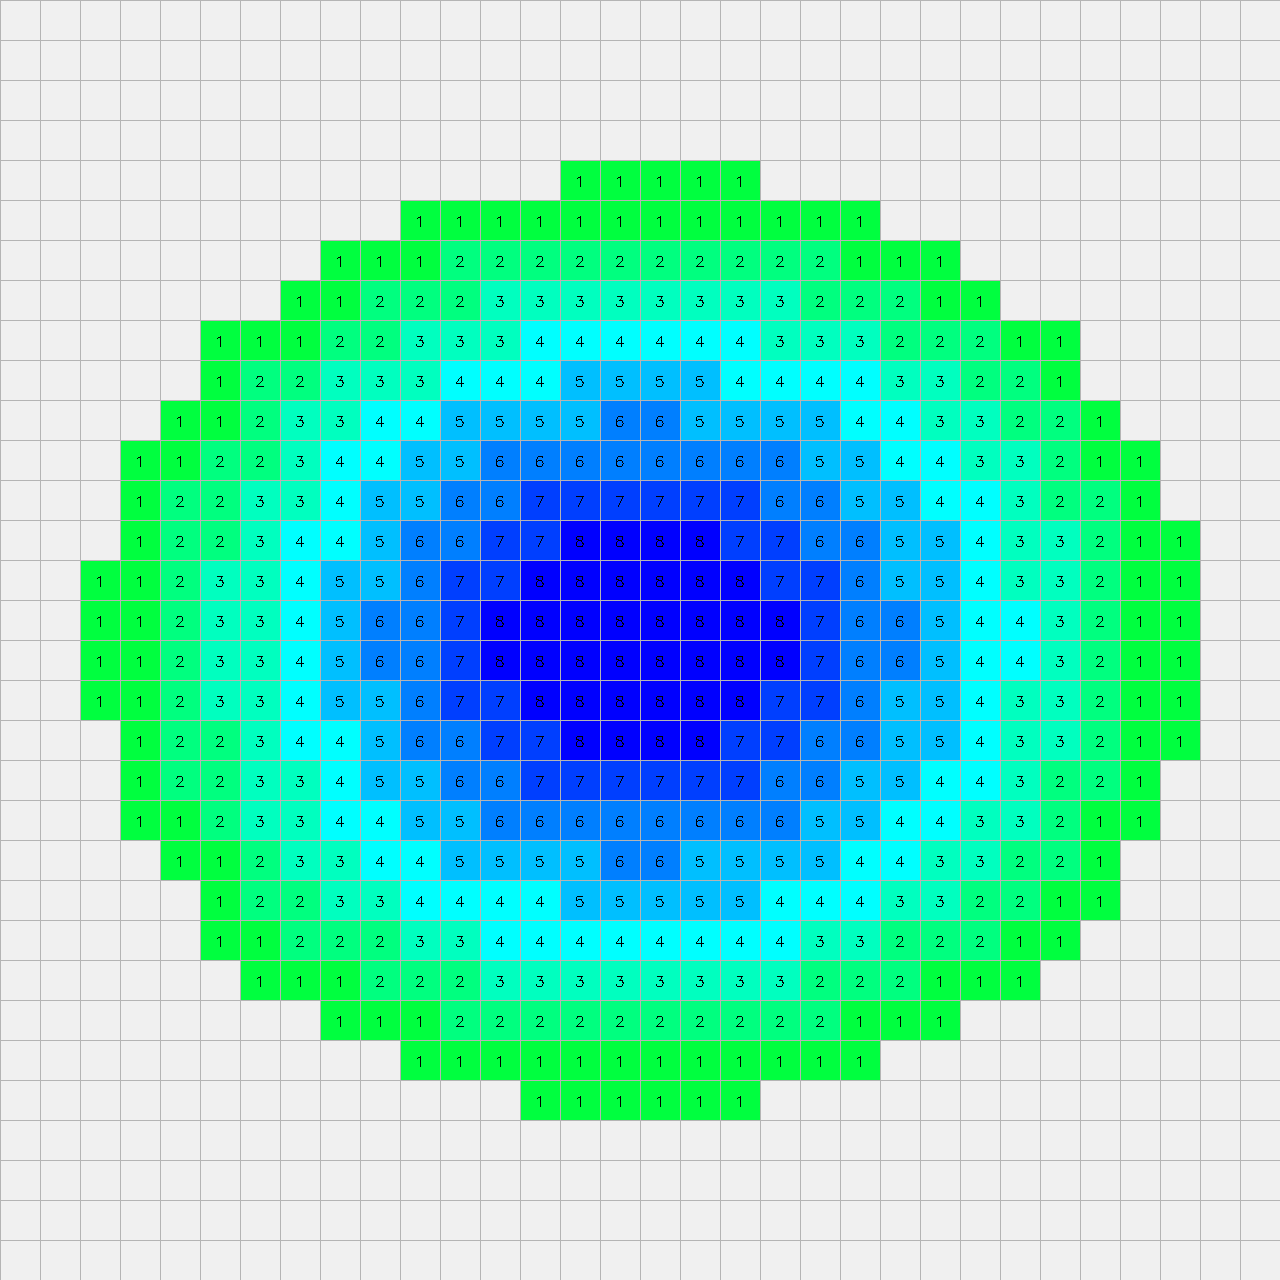
\includegraphics[width=\textwidth]{heightmap_visualization.png}
        \caption{Output: $32\times32$ height matrix visualization}
        \label{fig:heightmap}
    \end{minipage}
\end{figure}

% ============================================================
% Chapter 4: Control Layer
% ============================================================
\section{Control Layer}

The Control Layer is responsible for robot arm motion planning and block management. The core class is \texttt{TerrainBuilder}, implemented in \texttt{terrain\_builder.py}.

\subsection{Class Initialization}

\begin{pythoncode}[terrain\_builder.py: Core Class Initialization]
class TerrainBuilder(object):
    def __init__(self, grid_size=8, num_levels=8):
        # MoveIt interface initialization
        self.robot = moveit_commander.RobotCommander()
        self.scene = moveit_commander.PlanningSceneInterface()
        self.move_group = moveit_commander.MoveGroupCommander("panda_arm")
        
        # Terrain parameters
        self.grid_size = grid_size          # 32×32
        self.num_levels = num_levels        # Max 8 layers
        self.block_size = 0.02              # Block side length 2cm
        self.grid_spacing = 0.02            # Grid spacing 2cm
        self.approach_height = 0.10         # Safe approach height
        
        # State tracking
        self.heightmap = None
        self.current_heights = None
        self.blocks_placed = 0
        self.total_blocks = 0
\end{pythoncode}

\subsection{Control Workflow}

After the \texttt{terrain\_builder.py} node initializes, it executes the following steps sequentially:

\subsubsection{Initialization Phase}

\begin{itemize}
    \item Variable settings: block, grid
    \item Recognition module call: \texttt{contour\_to\_heightmap.py}
    \item Related node communication
    \item Visualization settings
\end{itemize}

\subsubsection{Robot Arm Motion Workflow and Position Control}

The robot arm motion workflow covers the complete path planning and position control from picking to placing:

\begin{enumerate}
    \item Up the block
    \item Block generating
    \item Down to grasp position
    \item Close the gripper
    \item Pick up
    \item Move with block
    \item 14\,cm above destination
    \item Loose the gripper
\end{enumerate}

The core pick function \texttt{pick\_from\_supply} is implemented as:

\begin{pythoncode}[terrain\_builder.py: Pick Block]
def pick_from_supply(self):
    # Move above the supply area
    pre_z = self.supply_z + self.approach_height
    self.center_block_above(self.supply_x, self.supply_y, pre_z)
    
    # Open gripper, descend precisely
    self.open_gripper()
    grasp_flange_z = self.supply_z - self._z_offset * self._grasp_zz
    self.cartesian_move_to_z(grasp_flange_z)
    
    # Close gripper to grasp block
    self.close_gripper()
    
    # Create marker that follows the gripper
    self._start_tracking(held_marker)
    
    # Remove collision object from supply area
    self.scene.remove_world_object(supply_name)
    
    # Lift up and return
    self.cartesian_move(self.approach_height + 0.05)
    return supply_name
\end{pythoncode}

The system achieves precise pick-and-place operations through position control, ensuring each block reaches its target location accurately. The core position control function \texttt{center\_block\_above} implements precise IK-based motion:

\begin{pythoncode}[terrain\_builder.py: Position Control]
def center_block_above(self, cx, cy, z_target):
    # Calculate flange target position (align block center to target point)
    flange_x = cx - self._z_offset * self._grasp_zx
    flange_y = cy - self._z_offset * self._grasp_zy
    flange_z = z_target - self._z_offset * self._grasp_zz
    
    # Use full-pose IK
    q = quaternion_from_euler(self.GRASP_ROLL, self.GRASP_PITCH, self.GRASP_YAW)
    pose = geometry_msgs.msg.Pose()
    pose.position.x = flange_x
    pose.position.y = flange_y
    pose.position.z = flange_z
    pose.orientation = q
    
    self.move_group.set_pose_target(pose)
    success = self.move_group.go(wait=True)
    self.move_group.clear_pose_targets()
    return success
\end{pythoncode}

For the final 14\,cm precise vertical descent, the system employs Cartesian path planning:

\begin{pythoncode}[terrain\_builder.py: Cartesian Path]
def cartesian_move_to_z(self, target_z):
    current = self.move_group.get_current_pose().pose
    target = copy.deepcopy(current)
    target.position.z = target_z
    
    # Compute Cartesian straight-line path
    (plan, fraction) = self.move_group.compute_cartesian_path(
        [target], 0.005, True)
    
    if plan and len(plan.joint_trajectory.points) > 0:
        return self.move_group.execute(plan, wait=True)
    return False
\end{pythoncode}

\subsubsection{Block Motion and Block Management}

\textbf{Block Motion Workflow:}

\begin{enumerate}
    \item Generate
    \item Move with arm
    \item Drop with $g$ acceleration
\end{enumerate}

\subsubsection{High-Frequency Block Tracking via TF2}

During transport, the system must keep the visual block marker precisely aligned with the gripper in RViz. The conventional approach — calling MoveIt's \texttt{get\_current\_pose()} — suffers from ROS topic latency and planning scene state locks, causing visible lag and "trailing" of the block marker.

To resolve this, the system directly queries the TF2 (Transform Framework 2) tree. TF2 is ROS's core component for maintaining coordinate frame relationships.

The \texttt{robot\_state\_publisher} node publishes transformations between all robot links at high frequency (default 100Hz), storing them in the \texttt{tf2\_buffer} for real-time queries.

The \texttt{TerrainBuilder} class initializes the TF2 buffer and listener as follows:

\begin{pythoncode}[terrain\_builder.py: TF2 Initialization]
# TF2 initialization — for high-frequency, low-latency transform lookups
self._tf_buffer = tf2_ros.Buffer()
self._tf_listener = tf2_ros.TransformListener(self._tf_buffer)
\end{pythoncode}

After a successful grasp, the system calls \texttt{\_start\_tracking} to launch a 50Hz timer. In the timer callback \texttt{\_tracking\_cb}, it queries the latest transform from the gripper frame \texttt{panda\_link8} to the world frame \texttt{planning\_frame} via \texttt{lookup\_transform}:

\begin{pythoncode}[terrain\_builder.py: TF2 High-Frequency Tracking]
def _start_tracking(self, marker):
    """Start tracking — marker follows the gripper via TF2 at 50Hz"""
    self._held_marker = marker
    self._block_held = True
    # 50Hz timer, querying TF every 20ms
    self._tracking_timer = rospy.Timer(
        rospy.Duration(0.02), self._tracking_cb)

def _tracking_cb(self, event):
    """Timer callback: retrieve real-time gripper pose via TF2 and update marker"""
    try:
        # Query the latest TF transform (rospy.Time(0) = latest available)
        transform = self._tf_buffer.lookup_transform(
            self.planning_frame,   # target frame (world)
            self.eef_link,         # source frame (gripper)
            rospy.Time(0))         # latest timestamp
        
        # Compute block center position (gripper position + fixed offset)
        q = transform.transform.rotation
        zx = 2.0 * (q.x * q.z + q.y * q.w)
        zy = 2.0 * (q.y * q.z - q.x * q.w)
        zz = 1.0 - 2.0 * (q.x * q.x + q.y * q.y)
        
        self._held_marker.pose.position.x = (
            transform.transform.translation.x + self._z_offset * zx)
        self._held_marker.pose.position.y = (
            transform.transform.translation.y + self._z_offset * zy)
        self._held_marker.pose.position.z = (
            transform.transform.translation.z + self._z_offset * zz)
        
        # Publish the updated marker
        self._held_marker_pub.publish(MarkerArray(markers=[self._held_marker]))
    except tf2_ros.LookupException:
        # TF not yet available — skip this frame silently
        pass
\end{pythoncode}

The key advantage of this approach is that TF2 lookups are essentially memory reads — they involve no ROS service calls or topic communication, yielding microsecond-level latency. Combined with the 50Hz refresh rate, the block marker follows the gripper with virtually zero lag, visually "sticking" to the gripper throughout the transport phase.

When the block reaches its destination and the gripper opens, the system calls \texttt{\_stop\_tracking} to shut down the timer and send a DELETEALL message to remove the tracking marker, completing the visual feedback loop for each pick-and-place cycle.

The gravity animation implementation in the \texttt{place\_block\_at} function:

\begin{pythoncode}[terrain\_builder.py: Gravity Drop Animation]
def _animate_fall(self, name, start_z, end_x, end_y, end_z, r, g, b):
    fall_dist = start_z - end_z
    g = 9.81  # gravitational acceleration
    t_total = sqrt(2.0 * fall_dist / g)
    dt = 0.03  # 30Hz refresh rate
    
    for step in range(steps + 1):
        t = step * dt
        z = start_z - 0.5 * g * t * t
        # Update Marker position
        fall_marker.pose.position.z = max(z, end_z)
        self._marker_pub.publish(MarkerArray(markers=[fall_marker]))
        rospy.sleep(dt)
\end{pythoncode}

\textbf{Block Management:}

\begin{itemize}
    \item Block count — \texttt{blocks\_placed} increments for each block placed
    \item Change block ID — \texttt{\_supply\_counter} increments for each new block generated
\end{itemize}

The \texttt{build\_terrain} function iterates layer by layer to construct the terrain, while managing block picking, placement, and counting throughout the process:

\begin{pythoncode}[terrain\_builder.py: Terrain Building Main Loop + Block Management]
def build_terrain(self):
    max_h = int(self.heightmap.max())
    
    # Build layer by layer
    for layer in range(1, max_h + 1):
        # Filter cells that need blocks in this layer
        cells = [(i, j) for i in range(self.grid_size)
                 for j in range(self.grid_size)
                 if self.heightmap[i, j] >= layer]
        # Sort from back to front (ensures arm approaches from the rear)
        cells.sort(key=lambda ij: -ij[0])
        
        for i, j in cells:
            # Pick a block from the supply area
            block_name = self.pick_from_supply()
            # Place the block at the target position
            self.place_block_at(block_name, i, j, layer)
            # Block management: spawn next supply block, update block count and ID
            self._spawn_supply_block()
            self.blocks_placed += 1  # Block count
            
            # Progress output
            if self.blocks_placed % 10 == 0:
                rospy.loginfo("PROGRESS: %d/%d blocks (%.1f%%)",
                               self.blocks_placed, self.total_blocks,
                               100.0 * self.blocks_placed / self.total_blocks)
\end{pythoncode}

% ============================================================
% Chapter 5: Experimental Results
% ============================================================
\section{Experimental Results}

After system integration and testing, the following results were achieved:

\begin{itemize}
    \item[$\checkmark$] Able to recognize simple contour terrain maps
    \item[$\checkmark$] Able to build a $32 \times 32 \times 8$ 3D terrain model
    \item[$\checkmark$] No planning errors in hundreds of pick-and-place cycles
\end{itemize}

\begin{figure}[H]
    \centering
    \begin{minipage}{0.45\textwidth}
        \centering
        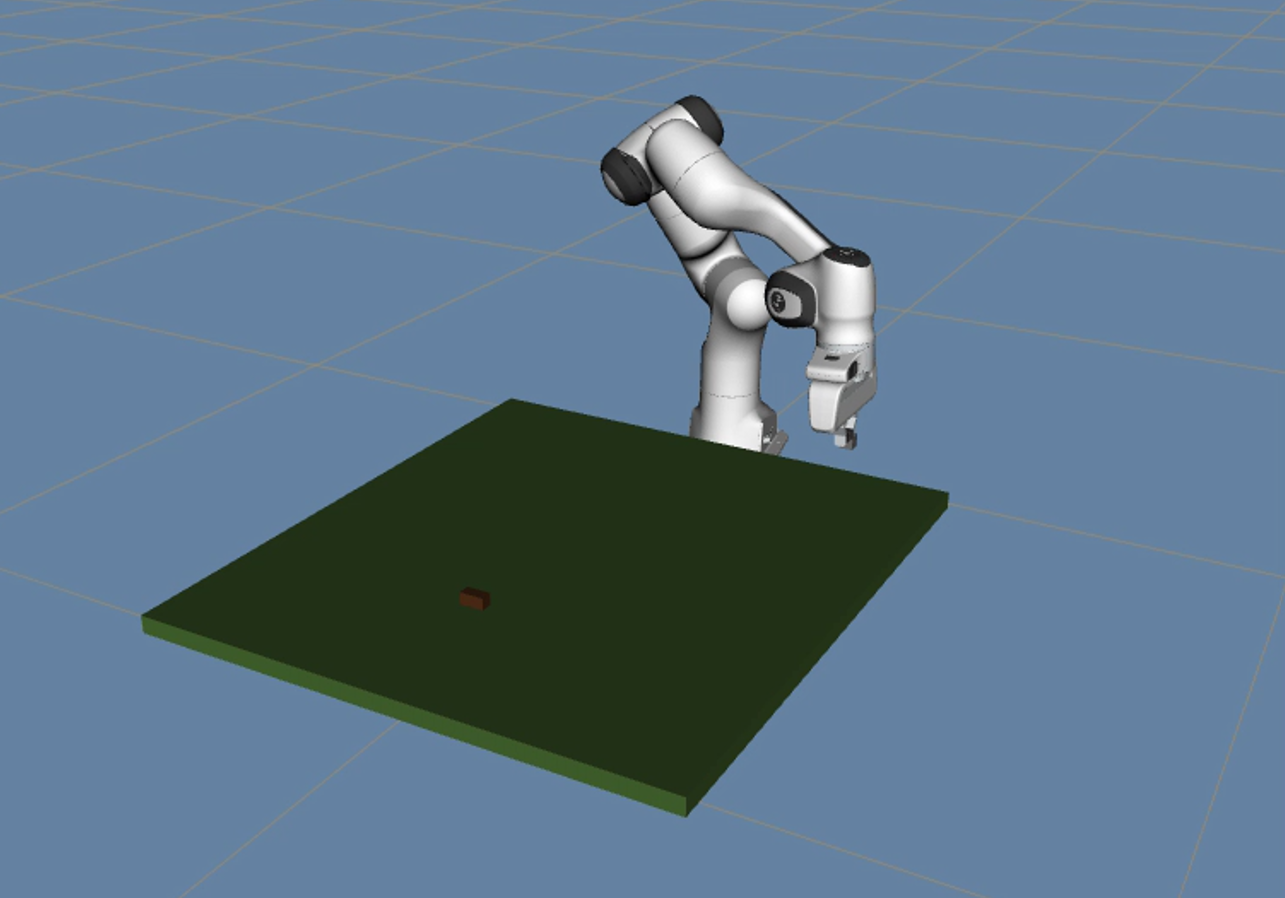
\includegraphics[width=\textwidth]{start.png}
        \caption{Building start}
        \label{fig:start}
    \end{minipage}
    \hfill
    \begin{minipage}{0.45\textwidth}
        \centering
        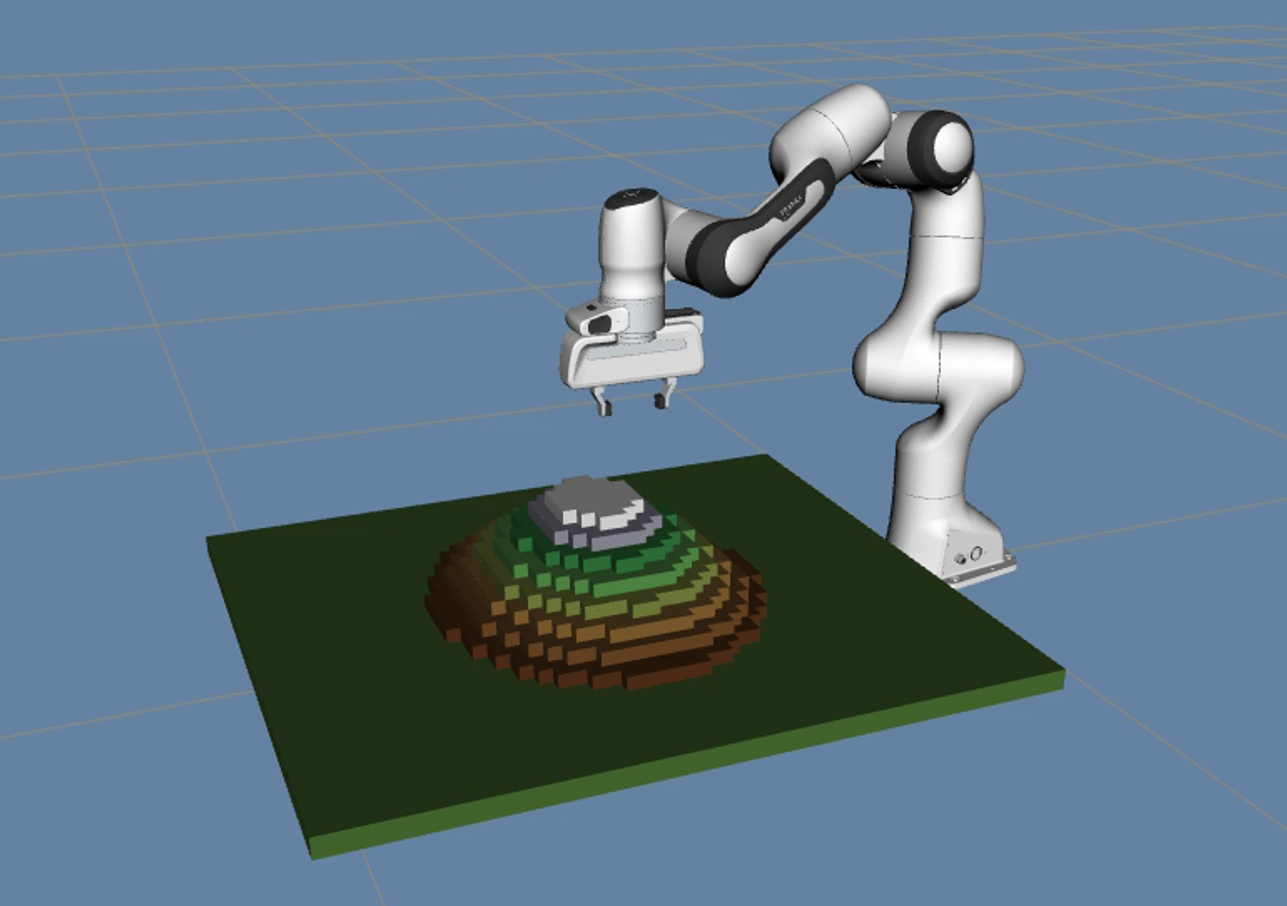
\includegraphics[width=\textwidth]{end.png}
        \caption{Building complete}
        \label{fig:end}
    \end{minipage}
\end{figure}

% ============================================================
% Chapter 6: Conclusion
% ============================================================
\section{Conclusion}

This project successfully implemented an automated 3D terrain construction system based on ROS Noetic and MoveIt. Using the Franka Emika Panda 7-joint robot arm, the system can automatically convert contour terrain maps into height matrices and stack precise terrain models layer by layer.

% ============================================================
% Appendix: Team Roles
% ============================================================
\section*{Appendix: Team Roles}
\addcontentsline{toc}{section}{Appendix: Team Roles}

\begin{table}[H]
    \centering
    \begin{tabular}{p{4cm} p{10cm}}
        \toprule
        \textbf{Role} & \textbf{Contributions} \\
        \midrule
        Software & Coding, simulation, and system integration \\
        Documentation & Report writing and presentation \\
        Media & Demo recording and visual assets \\
        \bottomrule
    \end{tabular}
\end{table}

\end{document}